\documentclass{article}

\usepackage[utf8]{inputenc}
\usepackage{amsmath}
\usepackage{graphicx}

\title{hello-\LaTeX}
\author{valorad }
\date{January 2020}

\begin{document}

\maketitle

\tableofcontents

\newpage

\section{Introduction}
% This section is very important
Welcome to this \textbf{presentation}. In this section, we will see how a program called \textit{superValleyStation} is boomed within \emph{0.1} seconds.

\section{Entertainment}

\subsection{TV}

\subsubsection{Talk-shows}

% \paragraph is like a heading

\paragraph{
Do various kinds of entertainment bring about happiness?
}

\ldots Y/n

\subparagraph{Why?}





\section{Mathtime}

\begin{equation}
    y_0 = x^{ \frac{3} {4} }
\end{equation}

\begin{equation}
   \frac {x^2 + a} {2x}
\end{equation}

\begin{equation}
   \sqrt[8]{x^3 + B}
\end{equation}

An inline version of equation is surrounded by double dollar signs like $+\infty$



\section{FigureTime}

Some figures will show here.

First, you will see a random cat in Figure \ref{fig:randomKit}.

An ancient research on cat predatory actions reveals that cats generally have high tendency on attacking rodents such as mice \cite{reis1973predatory}.

A recent study on the behavior of jungle cats also indicates that the cats are cats \cite{MARINATH2019112651}.


\begin{figure}
    \centering
    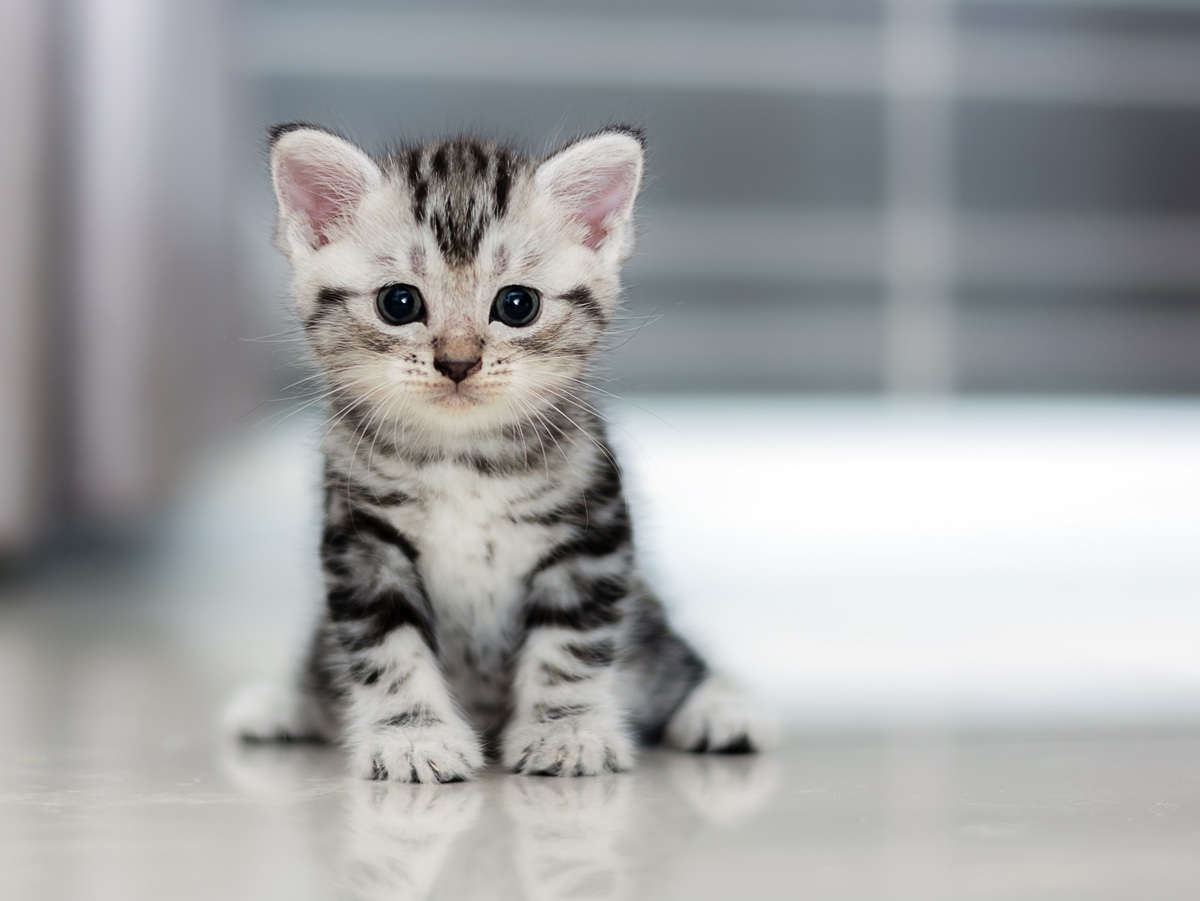
\includegraphics[width=0.5\textwidth]{images/kittenrandom.jpg}
    \caption{Random Kitten}
    \label{fig:randomKit}
\end{figure}


\section{Table time}

% Generate your table at https://www.tablesgenerator.com/latex_tables#

This section shows some tables.

First, some rubbish courses are shown in Table \ref{table:trashCourses}

\begin{table}[h]
\centering
\caption{Trash courses}
\label{table:trashCourses}
\begin{tabular}{|c|l|l|}
\hline
Course               & \multicolumn{1}{c|}{Difficulty} & \multicolumn{1}{c|}{Drop rate} \\ \hline
Lisa's cooking class & 60                              & 50                             \\ \hline
Boxing class         & 90                              & 0                              \\ \hline
\end{tabular}
\end{table}




\bibliographystyle{plain}
\bibliography{ref.bib}

\end{document}